\documentclass[5pt]{article}
\usepackage{mathptmx,amsmath}
\usepackage{pdfslide2,pause}
\usepackage{eurosym}
\usepackage[portuguese,english]{babel}
\usepackage{kerkis}
\usepackage{colortbl} % used to highlight row or columns of tables. http://www.tug.org/pracjourn/2007-1/mori/mori.pdf
\usepackage[small]{caption} % more option on http://www.dd.chalmers.se/latex/Docs/PDF/caption.pdf
\usepackage[tight,scriptsize]{subfigure}
\usepackage{lastpage}
\usepackage{chngcntr}
\usepackage[absolute,overlay]{textpos}
\usepackage{tabto}
\usepackage{animate}
%\usepackage{listings}
\captionsetup{labelformat=empty,skip=-0.8cm}

%\lstset{
%    language=Matlab,                % choose the language of the code
%    basicstyle=\ttfamily\tiny,       % the size of the fonts that are used for the code
%    numbers=none,                   % where to put the line-numbers
%    numberstyle=\tiny,              % the size of the fonts that are used for the line-numbers
%    stepnumber=1,                   % the step between two line-numbers. If it's 1 each line will be numbered
%    numbersep=5pt,                  % how far the line-numbers are from the code
%    backgroundcolor=\color{white},  % choose the background color. You must add \usepackage{color}
%    showspaces=false,               % show spaces adding particular underscores
%    showstringspaces=false,         % underline spaces within strings
%    showtabs=false,                 % show tabs within strings adding particular underscores
%    tab=\rightarrowfill,
%    frame=none,	                    % adds a frame around the code
%    tabsize=2,	                    % sets default tabsize to 2 spaces
%    captionpos=b,                   % sets the caption-position to bottom
%    breaklines=true,                % sets automatic line breaking
%    breakatwhitespace=false,        % sets if automatic breaks should only happen at whitespace
%    title=\lstname,                 % show the filename of files included with \lstinputlisting; also try caption instead of title
%    escapeinside={\%*}{*)},          % if you want to add a comment within your code
%    morekeywords={ifftshift,fftshift},
%    keywordstyle=\bfseries\color[rgb]{0,0,0.3},
%    commentstyle=\color[rgb]{0.133,0.5,0.133}
%}
%\lstset{
%    emph={function,end,for,if,while},
%    emphstyle=\bfseries\color[rgb]{0.6,0,0},
%}

\definecolor{itblue}{rgb}{0.0,0.0,0.5}
\definecolor{itred}{rgb}{0.82,0.18,0.24}
\newcommand{\pageNum}{
    \begin{picture}(0,0)(0,0)
        \put(-15,-390){
            \begin{minipage}{1.8cm}
            \end{minipage}
        }
    \end{picture}
}
\newcommand{\cb}[1]{{\color{itblue} #1}}%
\newcommand{\cred}[1]{{\color{itred} #1}}%
\newcommand{\bb}[1]{{\textbf{\color{itblue} #1}}}%
\newcommand{\br}[1]{{\textbf{\color{itred} #1}}}%
\renewcommand{\labelitemi}{\textcolor{itred}{\normalsize $\bullet$}}
\renewcommand{\labelitemii}{\textcolor{itblue}{$\bullet$}}
\newcommand{\mysection}[1]{\section*{\pageNum\color{itred}\sffamily #1}\vspace*{0.5cm}\overlay{it_1.png}\sffamily}%
\newcommand{\ITfootnote}[1]{\hspace{1.8cm}\begin{minipage}{13cm}\tiny{#1}\end{minipage}}
\newcommand{\edfaGain}{$G=\exp\left(\frac{\alpha}{2}L_{span}\right)$}
\newenvironment{reference}{
    \begin{textblock*}{0.7\textwidth}(32mm,137mm)\tiny\noindent\bgroup\color{black}
}
{
    \egroup\end{textblock*}
}


\graphicspath{{./Figures/}}
\pagestyle{title}

\hyphenpenalty=50000
\tolerance=10000

\setlength{\textheight}{1.5\textheight}

%%%%%%%%%%%%%%%%%%%%%%%%%%%%%%%%%%%%%%%%%%%%%%%%%%%%%%%%%%%%%%%%%%%%%%%%%%%%%%%%%%%%%%%%%%%%%%%%%%%
%%%%%%%%%%%%%%%%%%%%%%%%%%%%%%%%%%%%%%%%%%%%%%%%%%%%%%%%%%%%%%%%%%%%%%%%%%%%%%%%%%%%%%%%%%%%%%%%%%%

\begin{document}

%************************************************************************************************
%                                          SLIDE
%************************************************************************************************
\pagenumbering{roman}
\begin{titlepage}  \overlay{it_0.png}

\color{itblue} \sffamily \noindent \small
\hspace*{1cm}  Universidade de Aveiro\\ %Instituto\\ Superior T�cnico, Instituto de Telecomunica��es\\
\hspace*{1cm}  2017-2018\\ %Lisboa, 14th of February, 2013\\

\vspace*{1cm}
\begin{center}
    \color{black} \sffamily \noindent \Large
    \br{Quantum Oblivious Key Distribution with Discrete Variables\\}
\end{center}
\vspace{6mm}
\begin{center}
    \color{black}
    \textbf{Mariana Ferreira Ramos\\}
    {(marianaferreiraramos@ua.pt)}
\end{center}

\vspace{0.0mm}
\scriptsize
\begin{center}
Department of Electronics, Telecommunications and Informatics,\\
University of Aveiro, Aveiro, Portugal\\
Instituto de Telecomunica\c{c}\~{o}es, Aveiro, Portugal\\
\end{center}

\vspace{1.0cm}
\hspace*{13.2cm}\tiny \copyright 2005, it - instituto de telecomunica\c{c}\~{o}es\hfill

\end{titlepage}


\renewcommand{\headsep}{-25pt}
\pagenumbering{arabic}

%--------------------------------------------------------------------------------------------------
%------------ SLIDE -------------------------------------------------------------------------------

\mysection{ \\[-5mm]1-out-of-2 OT Protocol: starting conditions}\large
\vspace*{0mm}
\begin{itemize}
    \item {Alice has two messages $m_1$ and $m_2$ and Bob wants to know one of them, $m_b$, without Alice knowing which one, i.e. without Alice knowing $b$, and Alice wants to keep the other message private, i.e. without Bob knowing $m_{\bar{b}}$.}\\[-5mm]
    \item {In order to implement OT between two parties (Alice and Bob) they must be able to exchange continuously oblivious keys, i.e a QOKD system must exist between them.}
    \item {Two basis are required: $'+'$ rectilinear basis and $'\times'$ diagonal basis. Lets assume,}
    
    \begin{center}
    \begin{tabular}{c|c}
            & Basis "+" \\ \hline
         0 & $\to (0^{\circ})$ \\
         1 & $\uparrow (90^{\circ})$ \\
    \end{tabular}
    \quad
    \begin{tabular}{c|c}
          & Basis "$\times$" \\ \hline
         0 & $\searrow (-45^{\circ})$ \\
         1 & $\nearrow (45^{\circ})$ \\
    \end{tabular}

\end{center}
\end{itemize}



%--------------------------------------------------------------------------------------------------
%------------ SLIDE -------------------------------------------------------------------------------

\mysection{ \\[-5mm]Quantum Oblivious Key Distribution System (QOKD)}\large
The QOKD system enables two parties (Alice and Bob) to share a set of keys. These keys have the particularity of being half right and half wrong. Only Bob knows which are right and wrong keys.

\begin{description}
  \item[Step 1] Set for both Alice and Bob the block length $l$. Lets assume $l=16$. Lets assume Alice generates two sequences with $l$ bits:
      $$S_{A1'} = \{0,0,1,1,1,0,0,1,1,0,0,1,1,1,0,1 \},$$
      $$S_{A2'} = \{1,1,1,0,0,0,0,0,1,1,0,0,1,0,1,1 \}.$$
  
\end{description}

%--------------------------------------------------------------------------------------------------
%------------ SLIDE -------------------------------------------------------------------------------

\mysection{ \\[-5mm]Quantum Oblivious Key Distribution System (QOKD)}\large
\vspace*{0mm}
\begin{description}
  \item[Step 2] Alice sends to Bob throughout a quantum channel $l$ photons encoded using the basis defined in $S_{A1'}$ and according to the key bits defined in $S_{A2'}$.
  $$S_{AB} = \{ \uparrow,\uparrow,\nearrow,\searrow,\searrow, \to , \to, \searrow ,\nearrow ,\uparrow ,\to,\searrow,\nearrow,\searrow ,\uparrow ,\nearrow\} $$
  
  \item[Step 3] Bob also randomly generates $l=16$ bits, which are going to define his measurement basis. Lets assume:
  \begin{align*}
             S_{B1'} & = \{0 \ ,1 \ ,1 \ ,0 \ ,0 \ ,1 \ ,0 \ ,1 \ ,1 \ ,0 \ ,1 \ ,1 \ ,0 \ ,0 \ ,0 \ ,1 \  \} \\
                    & = \{ +,\times,\times,+,+,\times,+,\times, \times,+, \times, \times \,+,+,+,\times \}.
  \end{align*}
  
   Bob will get $l$ results, where "$-$"\space{ } corresponds to no clicks in Bob's detector, due to attenuation,
      $$S_{B2'} = \{1,-,\underline{0},0,-,1,\underline{1},-,1,-,1,0,1,1,\underline{0},1 \}.$$
  
\end{description}




%--------------------------------------------------------------------------------------------------
%------------ SLIDE -------------------------------------------------------------------------------

\mysection{ \\[-5mm]Quantum Oblivious Key Distribution System (QOKD)}\large
\vspace*{0mm}

\begin{description}
  \item[Step 4] Bob is going to send a "$-1$"\space{ } or a hash value (calculated by using SHA256 algorithm) to Alice for each measurement that he performed, thereby being "$-1$"\space{ } the measurements which correspond to no clicks. Bob will send to Alice the following set:
      
       $$S_{BH1}=\{{S}_{1},-1,{S}_{2},{S}_{3}, -1,{S}_{4},{S}_{5},-1,{S}_{6},-1,{S}_{7},{S}_{8},{S}_{9},{S}_{10},{S}_{11},{S}_{12} \}.$$

  \item[Step 5] After Alice has received $S_{BH1}$, she sends throughout a classical channel the basis which she has used to codify the photons updated with the information about the no received photons, $$S_{A1'} = \{0,-1,1,1,-1,0,0,-1,1,-1,0,1,1,1,0,1 \}$$.
\end{description}

%--------------------------------------------------------------------------------------------------
%------------ SLIDE -------------------------------------------------------------------------------

\mysection{ \\[-5mm]Quantum Oblivious Key Distribution System (QOKD)}\large
\vspace*{4mm}

\begin{description}
  \item[Step 5 - cont] Due to attenuation, the previous sets are reduced to the length $12$ and they shall be replaced by the following:
      $$S_{A1}=\{0,1,1,0,0,1,0,1,1,1,0,1 \},$$
      $$S_{A2}=\{1,1,0,0,0,1,0,0,1,0,1,1 \},$$
      $$S_{B1}=\{0,1,0,1,0,1,1,1,0,0,0,1 \},$$
      $$S_{B2}=\{1,\underline{0},0,1,\underline{1},1,1,0,1,1,\underline{0},1 \}$$
      Note that $S_{B2}$ still has errors.
  \item [Step 6] In order to know which photons were measured correctly, Bob does the operation $S_{B3}=S_{B1} \oplus S_{A1}$. He gets,
  $$S_{B3} = \{1,1,0,0,1,1,0,1,0,0,1,1 \}.$$

\end{description}

%--------------------------------------------------------------------------------------------------
%------------ SLIDE -------------------------------------------------------------------------------

\mysection{ \\[-5mm]Quantum Oblivious Key Distribution System (QOKD)}\large
\vspace*{0mm}
\begin{description}
  \item[Step 6 - cont] Bob has been building two pair of sets, one for the right basis,

      $$S_{B_{rp}}= \{1,2,5,6,8,11,12 \},$$ $$ S_{B_{rb}} = \{1,0,1,1,0,0,1 \},$$
      where $S_{B_{rp}}$ is the set of positions and $SB_{rb}$ is the set of bit values he measured for each position. The other pair is for photons he measured with the wrong basis and then he just guessed the values,
      $$S_{B_{wp}}= \{3,4,7,9,10 \},$$ $$S_{B_{wb}} = \{0,1,1,1,1 \},$$
      where $S_{B_{wp}}$ is the set of positions and $S_{B_{wb}}$ is the set of bit values he measured for each position.



\end{description}
%--------------------------------------------------------------------------------------------------
%------------ SLIDE -------------------------------------------------------------------------------

\mysection{ \\[-5mm]Quantum Oblivious Key Distribution System (QOKD)}\large
\vspace*{0mm}

 \begin{description}
   \item[Step 6 (cont)]   At this point, in order to test Bob's honesty and to estimate the \textit{QBER} of the channel, Alice is going to ask Bob to open some pairs of the Bob's sets. She must open a minimum number of right position in order to guarantee a minimum \textit{QBER}.
       Alice chooses some positions to open and tells Bob which positions she wants to open.
        Lets assume Alice has verified these pairs using the hash function committed by Bob and concluded that he is being honest and then she sends to Bob the \textit{QBER} estimated.

    Bob has the previous sets replaced by the following,
      \begin{align*}
        S_{B_{rp}} & = \{1,2,5,6,8 \} \\
        S_{B_{rb}} & = \{1,0,1,1,0 \} \\
        S_{B_{wp}} & = \{3,4,7,9 \} \\
        S_{B_{wb}} & = \{0,1,1,1 \}
      \end{align*}


 \end{description}

%--------------------------------------------------------------------------------------------------
%------------ SLIDE -------------------------------------------------------------------------------

\mysection{ \\[-5mm]Quantum Oblivious Key Distribution System (QOKD)}\large
\vspace*{0mm}

\begin{description}
  \item[Step 6 (cont)] Since some bits of $S_{B_{rb}}$ were wrongly measured, Bob must apply an error correction algorithm in order to correct the error due transmission. In this case, as there are two sets with wrong and right bits, Bob has to apply a modified version of Cascade Algorithm. He will apply the real cascade to $S_{B_{rb}}$ and a fake cascade version to $S_{B_{wb}}$.
      Lets assume that after applying the modified version of Cascade Bob gets,
      
      \begin{align*}
        S_{B_{rp}} & = \{1,2,5,6,8 \} \\
        S_{B_{rb}} & = \{1,1,0,1,0 \} \\
        S_{B_{wp}} & = \{3,4,7,9 \} \\
        S_{B_{wb}} & = \{0,1,1,0 \}
      \end{align*}
\end{description}




%--------------------------------------------------------------------------------------------------
%------------ SLIDE-------
\mysection{Quantum Oblivious Key Distribution System (QOKD)}\large
\vspace{0.4cm}
\begin{description}
  \item[Step 6 - cont] Bob has to test Alice's honesty during the cascade algorithm by analysing the $QBER$ sent by Alice and if it is a realistic value.
  
  \item[Step 7] When Alice sends to Bob a photons set, they are building a set of pairs (array positions and bit values which correspond to measured photons at Bob's side and to the key bit with the photon was encoded at Alice's side).
      The main goal is to guarantee that Bob has the same number of right and wrong pairs. In addition, they must know information about $t$.
      
       Since Bob has sent to Alice the information about the smallest set, in this example, Alice know that there are four pairs of wrong positions and five pairs of right positions. Alice must destroy one of the right pairs by asking Bob to open it. Therefore, at $t=8$ both know that there are the same number of right and wrong pairs thereby being the main goal guaranteed.
      
\end{description}

%--------------------------------------------------------------------------------------------------
%------------ SLIDE-------
\mysection{Quantum Oblivious Key Distribution System (QOKD)}\large
\vspace{0cm}


  
    \begin{figure}[hbt]
    	\centering
    	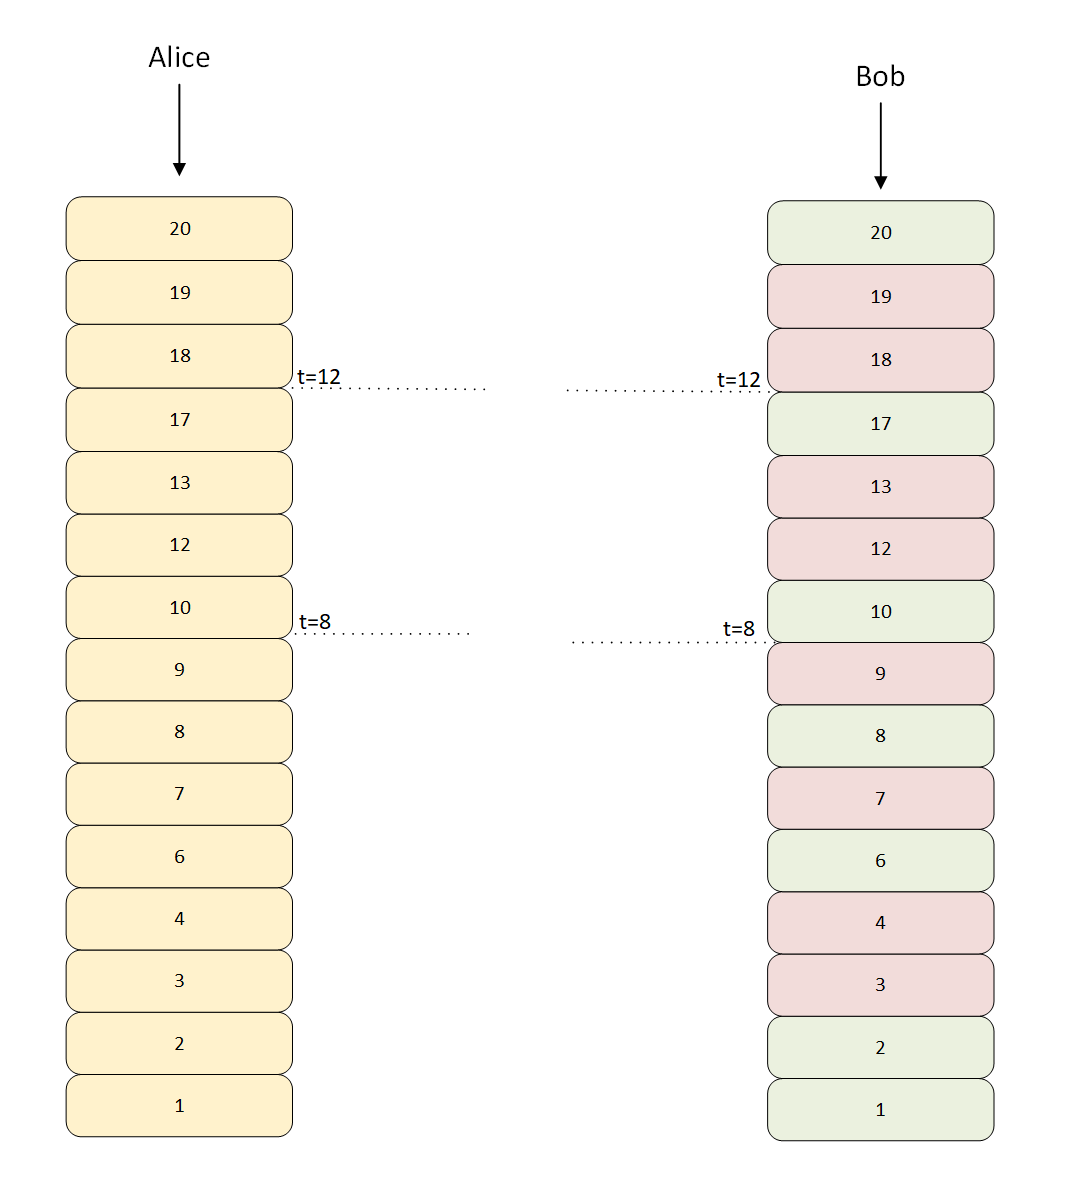
\includegraphics[width=1.0\textwidth, height=10cm]{./figures/alicebobkeys.png}
        	\caption{Alice and Bob key sets.}\label{alicebobkeys}
    \end{figure}



%--------------------------------------------------------------------------------------------------
%------------ SLIDE--------------------------------------------------------------------------------
\mysection{OT Protocol with QOKD system}\large
\vspace{0cm}
Alice sends two messages to Bob and he wants to know one of them. Alice does not know which message Bob wants and Bob only know the message he wants, i.e he does not know anything about the other message. Lets assume Alice send the following two messages with size $s=4$, $m_{0} = \{0 0 1 1\}$ and $m_{1} = \{0 0 0 1\}$. As $t=8$ Alice does not need to eliminate any bits.
\begin{description}
  \item[Step 1] Bob defines two sub-sets with size $s=4$:
  $$I_{0}=\{3,4,7,9 \},$$
  and $$I_{1}= \{1,2,6,8 \},$$ where $I_{0}$ is the sequence of positions in which Bob was wrong about basis measurement and $I_{1}$ is the sequence of positions in which Bob was right about basis measurement.


\end{description}

%--------------------------------------------------------------------------------------------------
%------------ SLIDE--------------------------------------------------------------------------------
\mysection{OT Protocol with QOKD system}\large
\vspace{0.4cm}
\begin{description}
  \item[Step 2] Bob sends to Alice the set $S_{b}$. Lets assume he wants to know $m_{0}$, therefore he sends $S_{0}=\{I_{1},I_{0} \}$. Alice is sure about Bob's honesty, since she knows he only has $4$ right basis to measure the photons. In addition, Alice cannot know which message Bob chose because she did not know the order that he sent the sets.
  \item[Step 3] Alice defines two encryption keys $K_{0}$ and $K_{1}$ using the values in positions defined by Bob in the set sent by him. Lets assume, $$K_{0}=\{1,1,1,0\}$$ $$K_{1}=\{0,0,0,1\}.$$ Alice does the following operations:
   $$m = \{m_{0}\oplus K_{0}, m_{1} \oplus K_{1} \}.$$

\end{description}
  


%--------------------------------------------------------------------------------------------------
%------------ SLIDE--------------------------------------------------------------------------------
\mysection{OT Protocol with QOKD system}\large
\vspace{0.4cm}
\begin{description}
  \item[Step 3 -cont ] Alice sends to Bob through a classical channel $$m=\{1,1,0,1,0,0,0,0\}.$$
  
  \item[Step 4] Bob uses $S_{B1\prime}$ values of positions given by $I_{1}$ and $I_{0}$ and does the decrypted operation. 
  
   \begin{table}[hbt]
        \centering
        \begin{tabular}{c|c c c c c c c c}
         $m$ & 1 & 1 & 0 & 1 & 0 & 0 & 0 & 0 \\
             & 1 & 1 & 1 & 0 & 0 & 1 & 1 & 0 \\ \hline
         $\oplus$ & 0 & 0 & 1 & 1 & 0 & 1 & 1 & 0 \\
        \end{tabular}
        \end{table}
    The first four bits corresponds to message 1 and he received $\{0,0,1,1\}$, which is the right message $m_{0}$ and $\{0,1,1,0\}$ which is a wrong message for $m_{1}$.
\end{description}





%-------------------------------------------------------------------
%------------ SLIDE ------------------------------------------------
\mysection{} \sffamily
\vspace{-10mm}
\large\centerline{E-mail: marianaferreiraramos@ua.pt}


\end{document}
